% Created 2024-09-21 Sat 15:07
% Intended LaTeX compiler: pdflatex
\documentclass[12pt]{article}
\usepackage[utf8]{inputenc}
\usepackage[T1]{fontenc}
\usepackage{graphicx}
\usepackage{longtable}
\usepackage{wrapfig}
\usepackage{rotating}
\usepackage[normalem]{ulem}
\usepackage{amsmath}
\usepackage{amssymb}
\usepackage{capt-of}
\usepackage{hyperref}
\usepackage[margin=1in]{geometry} \usepackage{amsmath}
\author{Jason Press}
\date{}
\title{Running in Circles to Measure Gravity}
\hypersetup{
 pdfauthor={Jason Press},
 pdftitle={Running in Circles to Measure Gravity},
 pdfkeywords={},
 pdfsubject={},
 pdfcreator={Emacs 29.4 (Org mode 9.7.11)}, 
 pdflang={English}}
\begin{document}

\maketitle
\begin{ABSTRACT}


In this lab, we used Newton's Second Law and a runner in uniform circular motion to calculate the acceleration due to Earth's gravity \(g\). When we measured the angle the runner makes with the ground when they run around a circle, we obtained a calculated value of \(g\) as \(9.6 \pm 0.25 \frac{\text{m}}{\text{s}^{2}}\). This value contains \(g\).
\end{ABSTRACT}
\section{Introduction}
\label{sec:org59e40f4}

The aim of this lab was to measure the acceleration due to Earth's gravity \(g\) by running in a circle.

When an object travels in uniform circular motion, it accelerates towards the center of the circle. When a human runs in a circle, it leans in the direction of the circle to turn. Since gravity pulls straight down, the force the human exerts on the ground when it leans at an angle \(\theta\) is has an \(\hat{z}\) and a \(\hat{r}\) component, where the \(\hat{z}\) component is equal and opposite to \(g\) and the \(\hat{r}\) component is equal to the centripetal acceleration. Here is the free body diagram of the human, represented as a singular point:

\begin{center}
\includegraphics[height=3.6in]{./bodyfbd.png}
\captionof{figure}{\label{fig:fbd}Free Body Diagram of a Human Running in a Circle}
\end{center}

Using Newton's Second Law, we can calculate the net force in the \(\hat{r}\) and \(\hat{z}\) directions as follows:

\begin{align}
\hat{r}: -|\vec{T}|\sin\theta = -m \frac{v^2}{R} \\
\hat{z}: -mg + |\vec{T}|\cos\theta = 0
\end{align}

Using some algebra, we can derive a formula for g:

\begin{align} \label{g}
g = \frac{v^2}{R\tan\theta}
\end{align}

Thus, by measuring the radius at which the human runs \(R\), the angle they lean at \(\theta\), and their velocity \(\frac{\Delta x}{\Delta t}\), we can calculate the acceleration due to Earth's gravity.

Another method to obtain \(g\) from Formula \ref{g} is to plot \(g\) as a function of \(v^2\) versus \(R\tan\theta\) with multiple data points, and the slope of the linear regression of the data points will be \(g\).
\section{Methods}
\label{sec:orgf936aa9}

To get a circle of radius \(R\), we picked a fixed point in a large, open area. Then, we placed one end of a roll tape at that fixed point. With the other end of the roll tape extended to a distance \(R\), we chose 10 meters, we placed a marker, a pole on a stand. Then, while keeping one end of the roll tape at the fixed point, we moved to a different point, approximately a fifth of a semicircle away from the first pole, and placed another pole. We did this until we had five (roughly) evenly spaced poles outlining a semicircle with a radius of 10 meters.

To get a \(\Delta x\), we took two bright markers (we used roll tapes) and placed them along the radius of the circle, at the middle pole, and placed them \(\Delta x\) meters apart. For this experiment, we chose 2 meters.

For the middle pole, we attached an arm and a heavy weight to the string. When the weight stopped moving, the string was perfectly vertical.

Finally, to get a \(\Delta t\) and \(\theta\), we had one camera (we used iPhone cameras) perpendicular to the two roll tapes and one camera in line with the two roll tapes, placed far enough away so that they could clearly capture a human running between the two roll tapes and without interfering with a human running along the semicircle.

Then, we drew straws to run. The runner ran along the semicircle traced by the poles at a constant speed, running such that their head was over the poles. During the run, the cameras recorded the runner passing between the roll tapes. The runner repeated this run five times, each time varying their speed.

To get \(\Delta t\) from the video, we took the timestamp where the runner's head passed the last marker and subtracted the timestamp where the runner's head passed the first marker. To get \(\theta\), we took the time where the runner was next to the middle pole, measured the angle using the Apple Photos video crop feature, rotating the guidelines such that they passed through the runner vertically, and then subtracting that angle measurement from the angle measurement relative to the string on the middle pole.

\begin{center}
\includegraphics[width=5.5in]{./setup.png}
\captionof{figure}{\label{fig:setup}Setup of the experiment}
\end{center}
\section{Results}
\label{sec:org878aba9}

Here were our measurements over five runs:

\begin{table}[htbp]
\caption{\label{table:measurements}Measurements}
\centering
\begin{tabular}{c|c|c|c|c}
\hline
Trial & \(\Delta t\) (s) & \(\theta\) (degrees) & \(R\tan\theta\) (m) & \(v^2\) \((\frac{\text{m}^{2}}{\text{s}^{2}})\)\\
\hline
1 & 0.44 & 12 & 2.12 & 20.7\\
2 & 0.48 & 11 & 1.94 & 17.4\\
3 & 0.39 & 14 & 2.49 & 26.3\\
4 & 0.38 & 17 & 3.06 & 27.7\\
5 & 0.32 & 22 & 4.04 & 39.1\\
\end{tabular}
\end{table}

Using linear regression through the origin, the calculated value of \(g\) is \(9.6 \pm 0.25 \frac{\text{m}}{\text{s}^{2}}\), which does contain the true value of \(g\). Here is the linear regression through the five data points:

\begin{center}
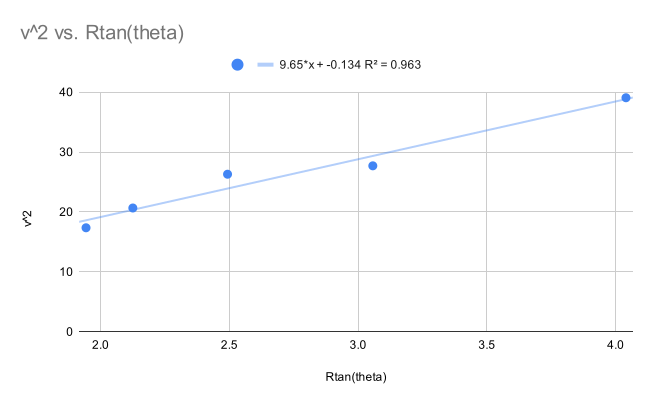
\includegraphics[width=6.5in]{./chart.png}
\captionof{figure}{\label{fig:graph}Linear regression of \(v^2\) versus \(R\tan\theta\)}
\end{center}

Please note that the regression line in Figure \ref{fig:graph} used is not through the origin, but it still gives a rough visual approximation of regression through the origin.
\section{Discussion}
\label{sec:org24241b1}

This value of \(g\) shocked our lab group. We did not expect this procedure to be as accurate as it was.

One major source of error for this lab was our runner. The original procedure for measuring \(\theta\) called for only the angle of the head to be measured. However, our runner ran with a tilted head, where he attempted to keep his head level. Thus, in order to obtain \(\theta\), we had to estimate the overall angle his body made with the ground.

Additionally, for estimating \(\Delta t\), we used an iPhone recording at 60 frames per second. As smooth as 60 fps video is, there was still uncertainty in picking the correct frame for the runner to have ``crossed'' the mark.

In our experiment, our runner also did not run perfectly along the arc laid out by the poles, although he tried his best to approximate it. What this means is our true value of \(R\) was not precisely 10 meters, but probably a little larger than 10 meters.

We account for all this error with the \texttt{LINEST} function in Google Sheets. One of the outputs of the \texttt{LINEST} function is standard error, which we used for our error.
\section{Sample Calculations}
\label{sec:org740433d}

We used a spreadsheet for all of our calculations. Each calculation uses specific cells, such as \texttt{D2}. To make them more generalized, I will use the notation \texttt{Dn} to represent all valid data cells in column \texttt{D}.

For the \texttt{g prediction} column, we used \texttt{1/(10*TAN(RADIANS(Dn)))*(Bn/An)\textasciicircum{}2}. We only used that for our own curiosity to see how accurate each measurement was relative to \(g\). To get \texttt{Rtan(theta)}, we used \texttt{(10)*TAN(RADIANS(Dn))}. Google Sheets' \texttt{TAN} function only takes in radians, and since we measured in degrees, we had to use the \texttt{RADIANS} function which converts an input in degrees to an output in radians. For \texttt{v\textasciicircum{}2}, we first calculated \texttt{speed} with \texttt{An/Bn}, and then squared it. To make sure we did our calculations correctly, we did the same thing with \texttt{(dx/dt)\textasciicircum{}2}, but just using the raw data with \texttt{(Bn/An)\textasciicircum{}2}, and it matched with \texttt{v\textasciicircum{}2}.

To get \(g\), we used the \texttt{LINEST} function in Google Sheets. In our spreadsheet, we used \texttt{LINEST(H2:H6, G2:G6, FALSE, TRUE)}. To make the chart used in Figure \ref{fig:graph}, we selected the data range and made a chart.

Here is the spreadsheet we used:

\begin{center}
\includegraphics[width=6.5in]{./spreadsheet.png}
\end{center}
\end{document}
